%# -*- coding: utf-8 -*-
%!TEX encoding = UTF-8 Unicode
%!TEX TS-program = xelatex
% vim:ts=4:sw=4
%
% 以上设定默认使用 XeLaTex 编译,并指定 Unicode 编码,供 TeXShop 自动识别

%第二回 
\chapter{俏潘娘簾下勾情 老王婆茶坊說技}


\begin{showcontents}{}

詞曰:

芙蓉面,冰雪肌,生來娉婷年已笄。裊裊倚門余。梅花半含蕊,似開還閉。初見簾邊,羞澀還留住;再過樓頭,款接多歡喜。行也宜,立也宜,坐也宜,偎傍更相宜。

話說當日武松來到縣前客店內,收拾行李鋪蓋,交土兵挑了,引到哥家。那婦人見了,強如拾得金寶一般歡喜,旋打掃一間房與武松安頓停當。武松吩咐土兵回去,當晚就在哥家歇宿。次日早起,婦人也慌忙起來,與他燒湯淨面。武松梳洗裹幘,出門去縣裡畫卯。婦人道:「叔叔畫了卯,早些來家吃早飯,休去別處吃了。」武松應的去了。到縣裡畫卯已畢,伺候了一早晨,回到家,那婦人又早齊齊整整安排下飯。三口兒同吃了飯,婦人雙手便捧一杯茶來,遞與武松。武松道:「交嫂嫂生受,武松寢食不安,明日撥個土兵來使喚。」那婦人連聲叫道:「叔叔卻怎生這般計較!自家骨肉,又不服事了別人。雖然有這小丫頭迎兒,奴家見他拿東拿西,蹀里蹀斜,也不靠他。就是撥了土兵來,那廝上鍋上灶不乾淨,奴眼裡也看不上這等人。」武松道:「恁的卻生受嫂嫂了。」有詩為證:

武松儀表豈風流,嫂嫂淫心不可收。
籠絡歸來家裡住,相思常自看衾稠。

話休絮煩。自從武松搬來哥家裡住,取些銀子出來與武大,買餅散茶果,請那兩邊鄰舍。都斗分子來與武松人情。武大又安排了回席,不在話下。過了數日,武松取出一匹彩色段子與嫂嫂做衣服。那婦人堆下笑來,便道:「叔叔如何使得!既然賜與奴家,不敢推辭。」只得接了,道個萬福。自此武松只在哥家宿歇。武大依前上街挑賣炊餅。武松每日自去縣裡承差應事,不論歸遲歸早,婦人頓茶頓飯,歡天喜地伏侍武松,武松倒覺過意不去。那婦人時常把些言語來撥他,武松是個硬心的直漢。

有話即長,無話即短,不覺過了一月有餘,看看十一月天氣,連日朔風緊起,只見四下彤雲密佈,又早紛紛揚揚飛下一天瑞雪來。好大雪!怎見得?但見:

萬里彤雪密佈,空中瑞祥飄簾。瓊花片片舞前簷。剡溪當此際,濡滯子猷船。頃刻樓台都壓倒,江山銀色相連。飛鹽撒粉漫連天。當時呂蒙正,窯內歎無錢。

當日這雪下到一更時分,卻早銀妝世界,玉碾乾坤。次日武鬆去縣裡畫卯,直到日中未歸。武大被婦人早趕出去做買賣,央及間壁王婆買了些酒肉,去武松房裡簇了一盆炭火。心裡自想道:「我今日著實撩鬥他他一撩鬥,不怕他不動情。」那婦人獨自冷冷清清立在簾兒下,望見武松正在雪裡,踏著那亂瓊碎玉歸來。婦人推起簾子,迎著笑道:「叔叔寒冷?」武松道:「感謝嫂嫂掛心。」入得門來,便把氈笠兒除將下來。那婦人將手去接,武松道:「不勞嫂嫂生受。」自把雪來拂了,掛在壁子上。隨即解了纏帶,脫了身上鸚哥綠紵絲衲襖,入房內。那婦人便道:「奴等了一早晨,叔叔怎的不歸來吃早飯?」武松道:「早間有一相識請我吃飯,卻才又有作杯,我不耐煩,一直走到家來。」婦人道:「既恁的,請叔叔向火。」武松道:「正好。」便脫了油靴,換了一雙襪子,穿了暖鞋,掇條凳子,自近火盆邊坐地。那婦人早令迎兒把前門上了閂,後門也關了。卻搬些煮熟菜蔬入房裡來,擺在桌子上。武松問道:「哥哥那裡去了?」婦人道:「你哥哥出去買賣未回,我和叔叔自吃三杯。」武松道:「一發等哥來家吃也不遲。」婦人道:「那裡等的他!」說猶未了,只見迎兒小女早暖了一注酒來。武松道:「又教嫂嫂費心。」婦人也掇一條凳子,近火邊坐了。桌上擺著杯盤,婦人拿盞酒擎在手裡,看著武松道:「叔叔滿飲此杯。」武松接過酒去,一飲而盡。那婦人又篩一杯酒來,說道:「天氣寒冷,叔叔飲過成雙的盞兒。」武松道:「嫂嫂自請。」接來又一飲而盡。武松卻篩一杯酒,遞與婦人。婦人接過酒來呷了,卻拿注子再斟酒放在武松面前。那婦人一徑將酥胸微露,雲鬟半裸,臉上堆下笑來,說道:「我聽得人說,叔叔在縣前街上養著個唱的,有這話麼?」武松道:「嫂嫂休聽別人胡說,我武二從來不是這等人。」婦人道:「我不信!只怕叔叔口頭不似心頭。」武松道:「嫂嫂不信時,只問哥哥就是了。」婦人道:「啊呀,你休說他,那裡曉得什麼?如在醉生夢死一般!他若知道時,不賣炊餅了。叔叔且請杯。」連篩了三四杯飲過。那婦人也有三杯酒落肚,哄動春心,那裡按納得住。欲心如火,只把閒話來說。武松也知了八九分,自己只把頭來低了,卻不來兜攬。婦人起身去燙酒。武松自在房內卻拿火箸簇火。婦人良久暖了一注子酒來,到房裡,一隻手拿著注子,一隻手便去武鬆肩上只一捏,說道:「叔叔只穿這些衣裳,不寒冷麼?」武松已有五七分不自在,也不理他。婦人見他不應,匹手就來奪火箸,口裡道:「叔叔你不會簇火,我與你撥火。只要一似火盆來熱便好。」武松有八九分焦燥,只不做聲。這婦人也不看武松焦燥,便丟下火箸,卻篩一杯酒來,自呷了一口,剩下半盞酒,看著武松道:「你若有心,吃我這半盞兒殘酒。」武松匹手奪過來,潑在地下說道:「嫂嫂不要恁的不識羞恥!」把手只一推,爭些兒把婦人推了一交。武松睜起眼來說道:「武二是個頂天立地噙齒戴發的男子漢,不是那等敗壞風俗傷人倫的豬狗!嫂嫂休要這般不識羞恥,為此等的勾當,倘有風吹草動,我武二眼裡認的是嫂嫂,拳頭卻不認的是嫂嫂!」婦人吃他幾句搶得通紅了面皮,便叫迎兒收拾了碟盞傢伙,口裡說道:「我自作耍子,不直得便當真起來。好不識人敬!」收了傢伙,自往廚下去了。正是:

落花有意隨流水,流水無情戀落花。

這婦人見勾搭武松不動,反被他搶白了一場。武松自在房中氣忿忿,自己尋思。天色卻是申牌時分,武大挑著擔兒,大雪裡歸來。推門進來,放下擔兒,進的裡間,見婦人一雙眼哭的紅紅的,便問道:「你和誰鬧來?」婦人道:「都是你這不不爭氣的,交外人來欺負我。」武大道:「誰敢來欺負你?」婦人道:「情知是誰?爭奈武二那廝。我見他大雪裡歸來,好意安排些酒飯與他吃,他見前後沒人,便把言語來調戲我。便是迎兒眼見,我不賴他。」武大道:「我兄弟不是這等人,從來老實。休要高聲,乞鄰舍聽見笑話。」武大撇了婦人,便來武二房裡叫道:「二哥,你不曾吃點心?我和你吃些個。」武松只不做聲,尋思了半晌,一面出大門。武大叫道:「二哥,你那裡去?」也不答應,一直只顧去了。武大回到房內,問婦人道:「我叫他又不應,只顧望縣裡那條路去了。正不知怎的了?」婦人罵道:「賊餛飩蟲!有甚難見處?那廝羞了,沒臉兒見你,走了出去。我猜他一定叫人來搬行李,不要在這裡住。卻不道你留他?」武大道:「他搬了去,須乞別人笑話。」婦人罵道:「混沌魍魎,他來調戲我,到不乞別人笑話!你要便自和他過去,我卻做不的這樣人!你與了我一紙休書,你自留他便了。」武大那裡敢再開口。被這婦人倒數罵了一頓。正在家兩口兒絮聒,只見武松引了個土兵,拿著條扁擔,逕來房內收拾行李,便出門。武大走出來,叫道:「二哥,做什麼便搬了去?」武松道:「哥哥不要問,說起來裝你的幌子,只由我自去便了。」武大那裡再敢問備細,由武松搬了出去。那婦人在裡面喃喃吶吶罵道:「卻也好,只道是親難轉債,人不知道一個兄弟做了都頭,怎的養活了哥嫂,卻不知反來咬嚼人!正是花木瓜空好看。搬了去,倒謝天地,且得冤家離眼睛。」武大見老婆這般言語,不知怎的了,心中反是放不下。自從武松搬去縣前客店宿歇,武大自依前上街賣炊餅。本待要去縣前尋兄弟說話,卻被這婦人千叮萬囑,吩咐交不要去兜攬他,因此武大不敢去尋武松。

說這武松自從搬離哥家,捻指不覺雪晴,過了十數日光景。卻說本縣知縣自從到任以來,卻得二年有餘,轉得許多金銀,要使一心腹人送上東京親眷處收寄,三年任滿朝覲,打點上司。一來卻怕路上小人,須得一個有力量的人去方好,猛可想起都頭武松,須得此人方了得此事。當日就喚武松到衙內商議道:「我有個親戚在東京城內做官,姓朱名勉,見做殿前太尉之職,要送一擔禮物,捎封書去問安。只恐途中不好行,若得你去方可。你休推辭辛苦,回來我自重賞。」武松應道:「小人得蒙恩相抬舉,安敢推辭!既蒙差遣,只此便去。」知縣大喜,賞了武松三杯酒,十兩路費。不在話下。

且說武松領了知縣的言語,出的縣門來,到下處,叫了土兵,卻來街上買了一瓶酒並菜蔬之類,逕到武大家。武大卻街上回來,見武松在門前坐地,交土兵去廚下安排。那婦人餘情不斷,見武松把將酒食來,心中自思:「莫不這廝思想我了?不然卻又回來怎的?到日後我且慢慢問他。」婦人便上樓去重勻粉面,再整雲鬟,換了些顏色衣服,來到門前迎接武松。婦人拜道:「叔叔,不知怎的錯見了,好幾日並不上門,叫奴心裡沒理會處。今日再喜得叔叔來家。沒事壞鈔做什麼?」武松道: 「武二有句話,特來要與哥哥說知。」婦人道:「既如此,請樓上坐。」三個人來到樓上,武松讓哥嫂上首坐了,他便掇杌子打橫。土兵擺上酒,並嗄飯一齊拿上來。武松勸哥嫂吃。婦人便把眼來睃武松,武松只顧吃酒。酒至數巡,武松問迎兒討副勸杯,叫土兵篩一杯酒拿在手裡,看著武大道:「大哥在上,武二今日蒙知縣相公差往東京幹事,明日便要起程,多是兩三個月,少是一月便回,有句話特來和你說。你從來為人懦弱,我不在家,恐怕外人來欺負。假如你每日賣十扇籠炊餅,你從明日為始,只做五扇籠炊餅出去,每日遲出早歸,不要和人吃酒。歸家便下了簾子,早閉門,省了多少是非口舌。若是有人欺負你,不要和他爭執,待我回來,自和他理論。大哥你依我時,滿飲此杯!」武大接了酒道:「兄弟見得是,我都依你說。」吃過了一杯,武松再斟第二盞酒,對那婦人說道:「嫂嫂是個精細的人,不必要武松多說。我的哥哥為人質樸,全靠嫂嫂做主。常言表壯不如裡壯,嫂嫂把得家定,我哥哥煩惱做什麼!豈不聞古人云:籬牢犬不入。」那婦人聽了這句話,一點紅從耳邊起,須臾紫漲了面皮,指著武大罵道:「你這個混沌東西。有甚言語在別處說,來欺負老娘!我是個不帶頭巾的男子漢,叮叮噹噹響的婆娘!拳頭上也立得人,胳膊上走得馬,不是那腲膿血搠不出來鱉!老娘自從嫁了武大,真個螞蟻不敢入屋裡來,什麼籬笆不牢犬兒鑽得入來?你休胡言亂語,一句句都要下落!丟下一塊瓦磚兒,一個個也要著地!」武松笑道:「若得嫂嫂做主,最好。只要心口相應。既然如此,我武松都記得嫂嫂說的話了,請過此杯。」那婦人一手推開酒盞,一直跑下樓來,走到在胡梯上發話道:「既是你聰明伶俐,恰不道長嫂為母。我初嫁武大時,不曾聽得有甚小叔,那裡走得來?是親不是親,便要做喬家公。自是老娘晦氣了,偏撞著這許多鳥事!」一面哭下樓去了。正是:

苦口良言諫勸多,金蓮懷恨起風波。
自家惶愧難存坐,氣殺英雄小二哥。

那婦人做出許多喬張致來。武大、武松吃了幾杯酒,坐不住,都下的樓來,弟兄灑淚而別。武大道:「兄弟去了,早早回來,和你相見。」武松道:「哥哥,你便不做買賣也罷,只在家裡坐的。盤纏,兄弟自差人送與你。」臨行,武松又吩咐道:「哥哥,我的言語休要忘了,在家仔細門戶。」武大道:「理會得了。」武松辭了武大,回到縣前下處,收拾行裝並防身器械。次日領了知縣禮物,金銀駝垛,討了腳程,起身上路,往東京去了,不題。

只說武大自從兄弟武松說了去,整整吃那婆娘罵了三四日。武大忍聲吞氣,由他自罵,只依兄弟言語,每日只做一半炊餅出去,未晚便回來。歇了擔兒,便先去除了簾子,關上大門,卻來屋裡坐的。那婦人看了這般,心內焦燥,罵道:「不識時濁物!我倒不曾見,日頭在半天裡便把牢門關了,也吃鄰舍家笑話,說我家怎生禁鬼。聽信你兄弟說,空生著卵鳥嘴,也不怕別人笑恥!」武大道:「由他笑也罷,我兄弟說的是好話,省了多少是非。」被婦人啐在臉上道:「呸!濁東西!你是個男子漢,自不做主,卻聽別人調遣!」武大搖手道:「由他,我兄弟說的是金石之語。」原來武鬆去後,武大每日只是晏出早歸,到家便關門。那婦人氣生氣死,和他合了幾場氣。落後鬧慣了,自此婦人約莫武大歸來時分,先自去收簾子,關上大門。武大見了,心裡自也暗喜,尋思道:「恁的卻不好?」有詩為證:

慎事關門並早歸,眼前恩愛隔崔嵬。
春心一點如絲亂,任鎖牢籠總是虛。

白駒過隙,日月如梭,才見梅開臘底,又早天氣回陽。一日,三月春光明媚時分,金蓮打扮光鮮,單等武大出門,就在門前簾下站立。約莫將及他歸來時分,便下了簾子,自去房內坐的。一日也是合當有事,卻有一個人從簾子下走過來。自古沒巧不成話,姻緣合當湊著。婦人正手裡拿著叉竿放簾子,忽被一陣風將叉竿刮倒,婦人手擎不牢,不端不正卻打在那人頭上。婦人便慌忙陪笑,把眼看那人,也有二十五六年紀,生得十分浮浪。頭上戴著纓子帽兒,金鈴瓏簪兒,金井玉欄杆圈兒;長腰才,身穿綠羅褶兒;腳下細結底陳橋鞋兒,清水布襪兒;手裡搖著灑金川扇兒,越顯出張生般龐兒,潘安的貌兒。可意的人兒,風風流流從簾子下丟與個眼色兒。這個人被叉竿打在頭上,便立住了腳,待要發作時,回過臉來看,卻不想是個美貌妖嬈的婦人。但見他黑鬒鬒賽鴉鴒的鬢兒,翠彎彎的新月的眉兒,香噴噴櫻桃口兒,直隆隆瓊瑤鼻兒,粉濃濃紅艷腮兒,嬌滴滴銀盆臉兒,輕裊裊花朵身兒,玉纖纖蔥枝手兒,一捻捻楊柳腰兒,軟濃濃粉白肚兒,窄星星尖翹腳兒,肉奶奶胸兒,白生生腿兒,更有一件,緊揪揪、白鮮鮮、黑裀裀,正不知是什麼東西。觀不盡這婦人容貌。且看他怎生打扮?但見:

%䯼 鬏 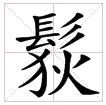
\includegraphics[width=20pt]{figures-char/diji.jpeg}%{髟狄}
頭上戴著黑油油頭髮䯼髻,一逕裡
{執足} %縶
出香雲,周圍小簪兒齊插。斜戴一朵並頭花,排草梳兒後押。難描畫,柳葉眉襯著兩朵桃花。玲瓏墜兒最堪誇,露來酥玉胸無價。毛青布大袖衫兒,又短襯湘裙碾絹紗。通花汗巾兒袖口兒邊搭剌。香袋兒身邊低掛。抹胸兒重重紐扣香喉下。往下看尖翹翹金蓮小腳,雲頭巧緝山鴉。鞋兒白綾高底,步香塵偏襯登踏。紅紗膝褲扣鶯花,行坐處風吹裙跨。口兒裡常噴出異香蘭麝,櫻桃口笑臉生花。人見了魂飛魄喪,賣弄殺俏冤家。

那人一見,先自酥了半邊,那怒氣早已鑽入爪窪國去了,變做笑吟吟臉兒。這婦人情知不是,叉手望他深深拜了一拜,說道:「奴家一時被風失手,誤中官人,休怪!」那人一面把手整頭巾,一面把腰曲著地還喏道:「不妨,娘子請方便。」卻被這間壁住的賣茶王婆子看見。那婆子笑道:「兀的誰家大官人打這屋簷下過?打的正好!」那人笑道:「倒是我的不是,一時衝撞,娘子休怪。」婦人答道:「官人不要見責。」那人又笑著大大地唱個喏,回應道:「小人不敢。」那一雙積年招花惹草,慣覷風情的賊眼,不離這婦人身上,臨去也回頭了七八回,方一直搖搖擺擺遮著扇兒去了。

風日晴和漫出遊,偶從簾下識嬌羞。
只因臨去秋波轉,惹起春心不自由。

當時婦人見了那人生的風流浮浪,語言甜淨,更加幾分留戀:「倒不知此人姓甚名誰,何處居住。他若沒我情意時,臨去也不回頭七八遍了。」卻在簾子下眼巴巴的看不見那人,方才收了簾子,關上大門,歸房去了。

看官聽說,這人你道是誰?卻原來正是那嘲風弄月的班頭,拾翠尋香的元帥,開生藥鋪複姓西門單諱一個慶字的西門大官人便是。只因他第三房妾卓二姐死了,發送了當,心中不樂,出來街上行走,要尋應伯爵到那裡去散心耍子。卻從這武大門前經過,不想撞了這一下子在頭上。卻說這西門大官人自從簾子下見了那婦人一面,到家尋思道:「好一個雌兒,怎能夠得手?」猛然想起那間壁賣茶王婆子來,堪可如此如此,這般這般:「撮合得此事成,我破費幾兩銀子謝他,也不值甚的。」於是連飯也不吃,走出街上閒遊,一直逕踅入王婆茶坊裡來,便去裡邊水簾下坐了。王婆笑道:「大官人卻才唱得好個大肥喏!」西門慶道:「乾娘,你且來,我問你,間壁這個雌兒是誰的娘子?」王婆道:「他是閻羅大王的妹子,五道將軍的女兒,問他怎的?」西門慶道:「我和你說正話,休要取笑。」王婆道:「大官人怎的不認得?他老公便是縣前賣熟食的。」西門慶道:「莫不是賣棗糕徐三的老婆?」王婆搖手道:「不是,若是他,也是一對兒。大官人再猜。」西門慶道:「敢是賣馉饳的李三娘子兒?」王婆搖手道:「不是,若是他,倒是一雙。」西門慶道:「莫不是花胳膊劉小二的婆兒?」王婆大笑道:「不是,若是他時,又是一對兒。大官人再猜。」西門慶道:「乾娘,我其實猜不著了。」王婆哈哈笑道:「我好交大官人得知了罷,他的蓋老便是街上賣炊餅的武大郎。」西門慶聽,跌腳笑道: 「莫不是人叫他三寸丁谷樹皮的武大麼?」王婆道:「正是他。」西門慶聽了,叫起苦來,說是:「好一塊羊肉,怎生落在狗口裡!」王婆道:「便是這般故事,自古駿馬卻馱癡漢走,美妻常伴拙夫眠。月下老偏這等配合。」西門慶道:「乾娘,我少你多少茶果錢?」王婆道:「不多,由他,歇些時卻算不妨。」西門慶又道: 「你兒子王潮跟誰出去了?」王婆道:「說不的,跟了一個淮上客人,至今不歸,又不知死活。」西門慶道:「卻不交他跟我,那孩子倒乖覺伶俐。」王婆道:「若得大官人抬舉他時,十分之好。」西門慶道:「待他歸來,卻再計較。」說畢,作謝起身去了。

約莫未及兩個時辰,又踅將來王婆門首,簾邊坐的,朝著武大門前半歇。王婆出來道:「大官人,吃個梅湯?」西門慶道:「最好多加些酸味兒。」王婆做了個梅湯,雙手遞與西門慶吃了。將盞子放下,西門慶道:「乾娘,你這梅湯做得好,有多少在屋裡?」王婆笑道:「老身做了一世媒,那討不在屋裡!」西門慶笑道: 「我問你這梅湯,你卻說做媒,差了多少!」王婆道:「老身只聽得大官人問這媒做得好。」西門慶道:「乾娘,你既是撮合山,也與我做頭媒,說頭好親事,我自重重謝你。」王婆道:「看這大官人作戲!你宅上大娘子得知,老婆子這臉上怎吃得那耳刮子!」西門慶道:「我家大娘子最好性格。見今也有幾個身邊人在家,只是沒一個中得我意的。你有這般好的,與我主張一個,便來說也不妨。若是回頭人兒也好,只是要中得我意。」王婆道:「前日有一個倒好,只怕大官人不要。」西門慶道:「若是好時,與我說成了,我自重謝你。」王婆道:「生的十二分人才,只是年紀大些。」西門慶道:「自古半老佳人可共,便差一兩歲也不打緊。真個多少年紀?」王婆道:「那娘子是丁亥生,屬豬的,交新年卻九十三歲了。」西門慶笑道:「你看這風婆子,只是扯著風臉取笑。」說畢,西門慶笑著起身去。

看看天色晚了,王婆恰才點上燈來,正要關門,只見西門慶又踅將來,逕去簾子底下凳子上坐下,朝著武大門前只顧將眼睃望。王婆道:「大官人吃個和合湯?」西門慶道:「最好!乾娘放甜些。」王婆連忙取一鍾來與西門慶吃了。坐到晚夕,起身道:「乾娘,記了帳目,明日一發還錢。」王婆道:「由他,伏惟安置,來日再請過論。」西門慶笑了去。到家甚是寢食不安,一片心只在婦人身上。就是他大娘子月娘,見他這等失張失致的,只道為死了卓二姐的緣故,倒沒做理會處。當晚無話。

次日清晨,王婆恰才開門,把眼看外時,只見西門慶又早在街前來回踅走。王婆道:「這刷子踅得緊!你看我著些甜糖抹在這廝鼻子上,交他抵不著。那廝全討縣裡人便宜,且交他來老娘手裡納些販鈔,嫌他幾個風流錢使。」原來這開茶坊的王婆,也不是守本分的,便是積年通慇勤,做媒婆,做賣婆,做牙婆,又會收小的,也會抱腰,又善放刁,端的看不出這婆子的本事來。但見:

開言欺陸賈,出口勝隋何。只憑說六國唇槍,全仗話三齊舌劍。只鸞孤鳳,霎時間交仗成雙;寡婦鰥男,一席話搬說擺對。解使三里門內女,遮莫九皈殿中仙。玉皇殿上侍香金童,把臂拖來;王母宮中傳言玉女,攔腰抱住。略施奸計,使阿羅漢抱住比丘尼;才用機關,交李天王摟定鬼子母。甜言說誘,男如封涉也生心;軟語調合,女似麻姑須亂性。藏頭露尾,攛掇淑女害相思;送暖偷寒,調弄嫦娥偷漢子。

這婆子正開門,在茶局子裡整理茶鍋,張見西門慶踅過幾遍,奔入茶局子水簾下,對著武大門首,不住把眼只望簾子裡瞧。王婆只推不看見,只顧在茶局子內煽火,不出來問茶。西門慶叫道:「乾娘,點兩杯茶來我吃。」王婆應道:「大官人來了?連日少見,且請坐。」不多時,便濃濃點兩盞稠茶,放在桌子上。西門慶道: 「乾娘,相陪我吃了茶。」王婆哈哈笑道:「我又不是你影射的,如何陪你喫茶?」西門慶也笑了,一會便問:「乾娘,間壁賣的是什麼?」王婆道:「他家賣的拖煎阿滿子,乾巴子肉翻包著菜肉匾食餃,窩窩蛤蜊面,熱燙溫和大辣酥。」西門慶笑道:「你看這風婆子,只是風。」王婆笑道:「我不風,他家自有親老公。」西門慶道:「我和你說正話。他家如法做得好炊餅,我要問他買四五十個拿的家去。」王婆道:「若要買炊餅,少間等他街上回來買,何消上門上戶!」西門慶道: 「乾娘說的是。」吃了茶,坐了一回,起身去了。

良久,王婆在茶局裡冷眼張著,他在門前踅過東,看一看,又轉西去,又復一復,一連走了七八遍。少頃,逕入茶房裡來。王婆道:「大官人僥倖,好幾日不見面了。」西門慶便笑將起來,去身邊摸出一兩一塊銀子,遞與王婆,說道:「乾娘,權且收了做茶錢。」王婆笑道:「何消得許多!」西門慶道:「多者乾娘只顧收著。」婆子暗道:「來了,這刷子當敗。且把銀子收了,到明日與老娘做房錢。」便道:「老身看大官人像有些心事的一般。」西門慶道:「如何幹娘便猜得著?」 婆子道:「有甚難猜處!自古入門休問榮枯事,觀著容顏便得知。老身異樣蹺蹊古怪的事,不知猜夠多少。」西門慶道:「我這一件心上的事,乾娘若猜得著時,便輸與你五兩銀子。」王婆笑道:「老身也不消三智五猜,只一智便猜個中節。大官人你將耳朵來:你這兩日腳步兒勤,趕趁得頻,一定是記掛著間壁那個人。我這猜如何?」西門慶笑將起來道:「乾娘端的智賽隋何,機強陸賈。不瞞乾娘說,不知怎的,吃他那日叉簾子時見了一面,恰似收了我三魂六魄的一般,日夜只是放他不下。到家茶飯懶吃,做事沒入腳處。不知你會弄手段麼?」王婆哈哈笑道:「老身不瞞大官人說,我家賣茶叫做鬼打更。三年前六月初三日下大雪,那一日賣了個泡茶,直到如今不發市,只靠些雜趁養口。」西門慶道:「乾娘,如何叫做雜趁?」王婆笑道:「老身自從三十六歲沒了老公,丟下這個小廝,沒得過日子。迎頭兒跟著人說媒,次後攬人家些衣服賣,又與人家抱腰收小的,閒常也會作牽頭,做馬百六,也會針灸看病。」西門慶聽了,笑將起來:「我並不知乾娘有如此手段!端的與我說這件事,我便送十兩銀子與你做棺材本。你好交這雌兒會我一面。」王婆便呵呵笑道:「我自說耍,官人怎便認真起來。你也!」且看下回分解。有詩為證:

西門浪子意猖狂,死下功夫戲女娘。
虧殺賣茶王老母,生交巫女會襄王。







\end{showcontents}
